% CHAPTER 3

\chapter{BACKGROUND}
\label{chp:background}
In this chapter background information is presented for the relevant topics to this thesis study. Topics are mentioned starting with the building blocks and then approaches with the order of their usage in the methodology presented in this thesis study. Firstly, event logs and process models are mentioned with their mathematical formalization and background. Following these, process discovery approaches are explained and then performance analysis methodologies are presented. Then, machine learning and clustering topics are mentioned. Finally, mismatch patterns in process models are presented. All topics in this chapter are limited to the scope of this thesis study with the aim of constructing a necessary background.

\section{Event Log}
\label{sec:event-log}
Event logs are the main inputs to any process mining methodology including this thesis study and they include information related to real life activities. Event logs which are the outputs of the software systems like Enterprise Resource Planning (ERP) or Business Process Management (BPM) have common properties that are also assumed in the literature as the properties of event logs. General structure of event logs includes multiple layers as diagrammed in Figure~\ref{fig:event-log-structure}. Processes have cases which are simply single process instances. Within each case, there are events that are generally represents a sequence of activities performed. Each event is enhanced with the attributes such as timestamps, resource assignments and other contextual data. A fragment of this structure is presented in Table~\ref{table:event-log-loan} for the Loan Application Process \cite{loan-app-data}, which shows the footprints of a financial organization that provides consumer credits \cite{buijs2013improving}. In the table, each line represents an event with its attributes which are collected under cases to form a complete event log. 
\begin{figure}
  \centering
  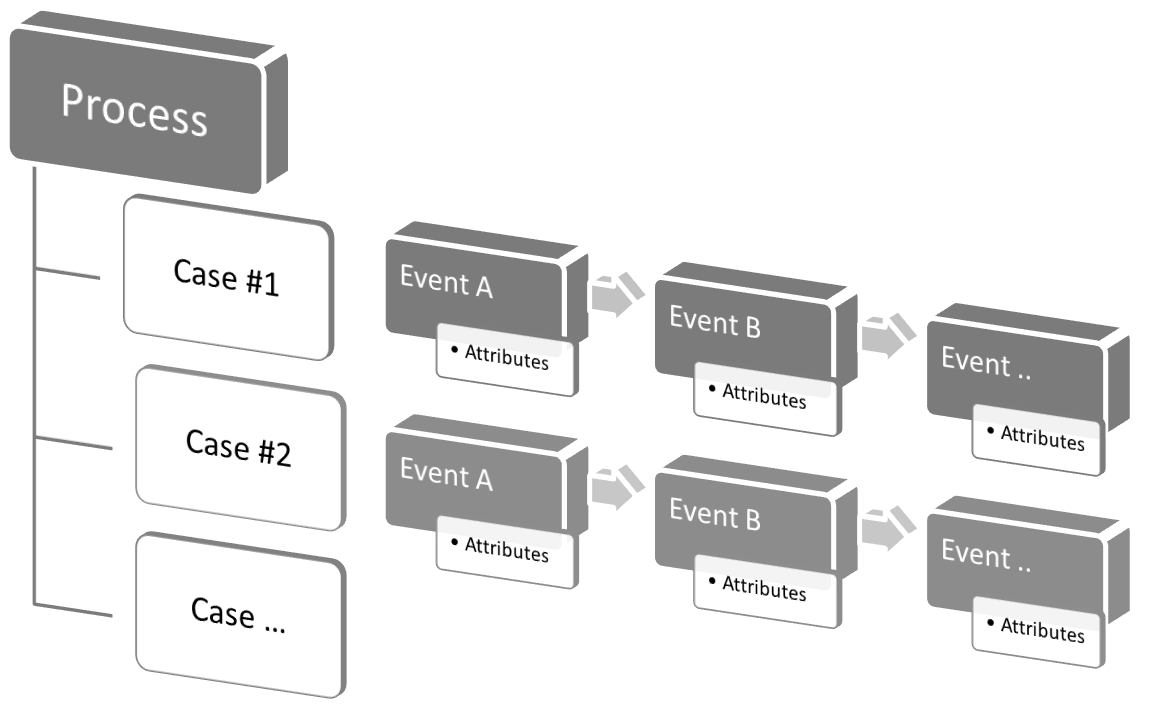
\includegraphics[width=\textwidth]{3_background/event_log_structure}
  \caption{Structure of Event Logs}
  \label{fig:event-log-structure}
\end{figure}

\begin{table}[h]
\centering
\caption{Fragment of event log from Loan Application Process (Variation \#1)}
\label{table:event-log-loan}
\begin{tabular}{@{}llccc@{}}
\toprule
\multicolumn{5}{c}{\textbf{Event Log}}                                                                  \\ \midrule
                        &                         & \multicolumn{3}{c}{\textbf{Attributes}}             \\ \midrule
                        & \textbf{Event}          & \textbf{Date} & \textbf{Time} & \textbf{Transition} \\ \midrule
\textbf{Case \#1}       & Register Application    & 16.04.2013    & 14:37:27      & Complete            \\ \midrule
                        & Check Credit            & 16.04.2013    & 14:41:19      & Complete            \\ \midrule
                        & Check System            & 16.04.2013    & 14:47:35      & Complete            \\ \midrule
                        & Calculate Capacity      & 16.04.2013    & 14:50:21      & Complete            \\ \midrule
                        & Accept                  & 16.04.2013    & 14:53:22      & Complete            \\ \midrule
                        & Send decision e-mail    & 16.04.2013    & 14:55:11      & Complete            \\ \midrule
\textbf{Case \#2}       & Register Application    & 16.04.2013    & 16:28:19      & Complete            \\ \midrule
                        & Check Credit            & 16.04.2013    & 16:36:22      & Complete            \\ \midrule
                        & Check System            & 16.04.2013    & 16:43:10      & Complete            \\ \midrule
                        & Calculate Capacity      & 16.04.2013    & 16:52:40      & Complete            \\ \midrule
                        & Reject                  & 16.04.2013    & 16:53:53      & Complete            \\ \midrule
                        & Send decision e-mail    & 16.04.2013    & 17:01:32      & Complete            \\ \midrule
\multicolumn{1}{c}{...} & \multicolumn{1}{c}{...} & ...           & ...           & ...                 \\ \bottomrule
\end{tabular}
\end{table}

Event log structure and related notions are formalized in \cite{van2011process} as following:
  \theoremstyle{definition}
  \begin{definition}{}
  (Event and Event Attributes) Let \textit{E} be the universe of events which include all possible event identifiers and in this universe any event \textit{e} $\in$ \textit{E}. Events are enhanced with contextual information, namely attributes. For any event \textit{e} $\in$ \textit{E} and attribute \textit{A}, $\#_\textit{A}(\textit{e})$ is the value of the attribute \textit{A} for event \textit{e}. Possible attributes for events include timestamps, people and resource assignments, transaction types and other contextual data.
  \end{definition}
  \theoremstyle{definition}
  \begin{definition}{}
  (Case and Case Attributes) Let \textit{C} be the universe of cases which include all possible case identifiers and in this universe any case \textit{c} $\in$ \textit{C}. Like events, cases are also enhanced with contextual information, namely attributes. For any case \textit{c} $\in$ \textit{C} and attribute \textit{A}, $\#_\textit{A}(\textit{c})$ is the value of the attribute \textit{A} for case \textit{c}. Each case has at least one attribute which is trace.
  \end{definition}
  \theoremstyle{definition}
  \begin{definition}{}
  (Trace) Trace is a sequence of event \textit{t} $\in$ ${E}^{*}$ such that each event is restricted to occur only once.
  \end{definition}
  \theoremstyle{definition}
  \begin{definition}{}
  (Event Log) Event log is set of cases \textit{L} $\subseteq$ \textit{C} such that each event occurs at most once in the event log.
  \end{definition}

In this study, event logs from different organizations are exploited, thus organization related attributes are used for cases. Within these event logs, traces of cases for each organization are used to discover underlying process models. In addition, timestamps and resource related attributes of events are used to collect performance related data for further analysis.

\section{Process Modeling}
\label{sec:process-modeling}
Process modeling is the foundation of process management applications and main tools of people in this profession. Although process modeling can be defined with informal process workflows to document procedures, there are a number of formalized notations which are more suitable to cross-applicability and mathematical analysis. In the control-flow view of process modeling, a process model is aimed to give decisions on which activities to take place with their orders. In this study, control-flow of process models are used to find mismatch patterns between different organizations that execute the same activities. Considering the scope of this  thesis, only Petri nets, Workflow Nets and Business Process Modeling Notation (BPMN) will be presented in this section. 

\subsection{Petri Nets}
\label{sec:petri-nets}
Petri net is a mathematical modeling language that is aimed to describe concurrent systems. Graphical notation of Petri nets seems intuitive and simple; however, it is powerful in terms of being executable and applicability of analysis techniques \cite{vanderAalst:2011:MBP:2000715}. Petri nets are directed bipartite graphs where \textit{nodes} represent transitions and \textit{places} represent conditions. Structure represented by Petri nets is static and the state of the net is described by placing \textit{tokens}, namely the process of \textit{marking}. Formalization of Petri nets are explained in \cite{reisig1998lectures} as following:
\theoremstyle{definition}
\begin{definition}{}
(Petri Nets) A \textit{Petri net} is a triplet $N = (P, T, F)$ where $P$ is finite set of \textit{places}, $T$ is finite set of \textit{transitions} and $F$ is set of \textit{flow relations} where:
\begin{enumerate}
  \item (Separation) $P \cap T = \varnothing$
  \item (Flow relation) $F \subseteq (P \times T) \cup (T \times P)$
\end{enumerate}
\end{definition}

\subsection{Workflow Nets}
\label{sec:workflow-nets}
Process models in the real life have additional properties to be executable and they are defined in the Workflow net formalization, which is simply a subset of Petri nets. These additional properties can be formalized as following \cite{van2013discovering}:
\theoremstyle{definition}
\begin{definition}{}
(Workflow Nets) Let $N = (P, T, F)$ be a Petri net and $t$ is a new identifier not in $P \cup T$. $N$ is a workflow net (WF-net) if and only if:
\begin{enumerate}
  \item (Start Node) $P$ contains a \textit{source place i} where no token can be fired to.
  \item (End Node) $P$ contains a \textit{sink place o} where no token can be fired from.
  \item (Connectedness) $\bar{N} = (P, T \cup \{t\}, F \cup \{(o,t),(t, i)\})$ is strongly connected; in other words, there is a directed path between any pair of nodes in $\bar{N}$.
\end{enumerate}
\end{definition}

In simple terms, a Workflow net is a Petri net with a source place to start the process and a sink place to end; furthermore, all nodes are on a path from source place to sink place \cite{van1998application}.  In order to illustrate this formalization, the Workflow net for the event log mentioned in Section~\ref{sec:event-log} is presented in Figure~\ref{fig:loan-petri-net}. In the figure, places are indicated by circles, transitions are indicated by rectangles, and flow relations are represented by arcs. 
\begin{figure}
  \centering
  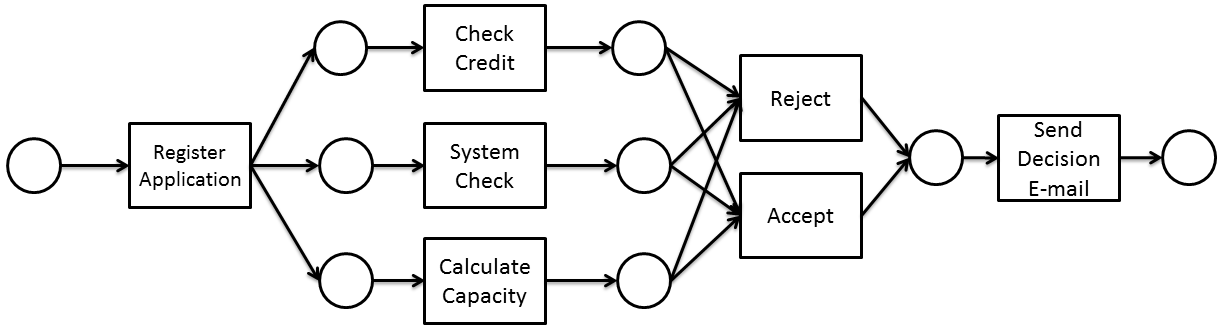
\includegraphics[width=\textwidth]{3_background/loan-petri-net}
  \caption{Workflow net of Loan Application Process (Variation \#1)}
  \label{fig:loan-petri-net}
\end{figure}

Workflow nets are representatives of real life processes; however, they can result with processes including deadlocks, live-locks and never-reached activities. In order to avoid process models from these problems, soundness definition is suggested in \cite{van1998application} and it is simplified as following with the context of this thesis:
\theoremstyle{definition}
\begin{definition}{}
(Soundness) Let $N$ be a Workflow net and it is sound if and only if:
\begin{enumerate}
  \item  (Safeness) Places cannot hold more than one tokens at the same time.
  \item  (Proper completion) Any marking of net can reach to sink place.
  \item  (Absence of dead tasks) Net does not contain any dead transitions.  
\end{enumerate}
\end{definition}

In this thesis, Workflow nets are used to discover and present underlying process models of different organizations. Considering the applicability of well-known process mining algorithms on Workflow nets and implementations in ProM Framework \cite{verbeek2010prom}, Workflow nets are used as the notation for discovery and analysis.

\subsection{Business Process Modeling Notation (BPMN)}
\label{sec:bpmn} 
Business Process Modeling Notation (BPMN) is one of the most popular and widely used modeling language implemented by many vendors. In addition to its popularity, this notation is standardized by the Object Management Group (OMG) since 2004. In this notation, atomic activities are named as \textit{tasks} and routing decision logic is implemented by \textit{gateways}. These gateways include split and join gateways with AND, OR and XOR logic operations. In addition, deferred choice pattern is implemented by \textit{event-based XOR gateway} in BPMN to handle race conditions between tasks that are running parallel \cite{van2003workflow}. Since the primary goal of BPMN is to provide a standardized notation that is easy to understand by business stakeholders, in this study resulting nets are converted to BPMN diagrams for visual analysis by the plugin implemented in ProM \cite{kalenkovaprocess}. BPMN diagram of the Workflow net from Figure~\ref{fig:loan-petri-net} is presented in Figure~\ref{fig:loan-bpmn}. As can be seen from the diagram, gateways help to understand the relations and dependencies of the tasks.

\begin{figure}
  \centering
  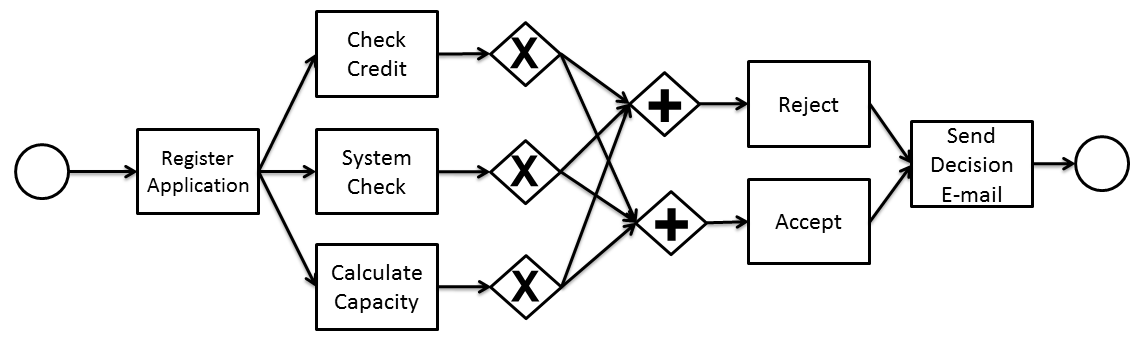
\includegraphics[width=\textwidth]{3_background/loan-bpmn}
  \caption{Process Model of Loan Application Process  (Variation \#1) using BPMN}
  \label{fig:loan-bpmn}
\end{figure}

\todo{checked until here!}
\section{Process Discovery}
\label{sec:process-discovery}
In process mining field, one of the most challenging task is to construct a process model based on the behavior in the event logs, namely process discovery. Many process discovery algorithms are proposed to address different challenges in process discovery and using different notations. However, in this thesis focus of the study is learning from the cross-organizational process mining rather than address all process discovery challenges. With this reasoning, Inductive Process Mining \cite{leemans2013discovering} is selected as appropriate since it is simple, highly applicable and configurable. In the literature, its derivatives which handles infrequent behaviors \cite{leemans2014discoveringinfrequent}; incomplete logs \cite{leemans2014discoveringincomplete}; and model optimization \cite{weidlich2012profiles} are also available.  

\textit{Inductive Miner (IM)}, which is proposed as an extensible framework in \cite{leemans2013discovering}, aims to discover block-structured process models that are sound and well-fitting to the behavior represented in event log. In addition, this approach focuses on creating rediscoverable models that is a key attribute in this study. Formalization of the key points in the study \cite{leemans2013discovering} are as following:

\theoremstyle{definition}
\begin{definition}{}
(Block-structured Workflow Nets) Block-structured WF-nets are subset of WF-nets where the workflow can be divided recursively into  parts with single entry and exit points.  
\end{definition}

\theoremstyle{definition}
\begin{definition}{}
(Rediscoverability) Let a process is expressible by a model $M$ which is unknown priori. Given a log $L$ of $M$, $L$ is a subset of language used to describe model $M$. $M$ is isomorphic-rediscoverable from $L$ by mining algorithm $B$ if and only if $M \in B(L)$.
\end{definition}
 
Framework developed in the study \cite{leemans2013discovering} uses a divide-and-conquer approach to discover subprocesses of sublogs obtained by splitting the event log. Main steps of the algorithm are listed as following:
\begin{enumerate}
  \item Activity Sets: Split the \textit{activities} in log to disjoint sets.
  \item Sublogs: Split the \textit{log} by using \textit{activity sets}.
  \item Recursive Mining: Mine sublogs with these steps until a sublog contains only single activity.
\end{enumerate}

In the study \cite{leemans2013discovering}, an algorithm based on this framework is presented that guarantees returning a sound and fitting process model in finite time. Therefore, this framework is selected as appropriate and its extension that can handle infrequent behavior is used within this thesis study to address challenges of different event logs. In real life, most of the cases in the events are samples of frequent behavior; however, there are also infrequent behaviors according to the nature of process execution environment. In real life, these different paths are used infrequently; however, their effect in discovery is still significant. \textit{Inductive Miner Infrequent (IMi)} is proposed in \cite{leemans2014discoveringinfrequent} as an extension to \textit{Inductive Miner} to handle noise in the event logs. By filtering the infrequent behavior, it is aimed that \textit{IMi} succeeds with improved models discovered. After each recursive step of \textit{IM}, filtering is applied if the discovered model is a flower model which represents infrequent behavior. Basic idea behind filtering is setting a user-defined threshold between 0 to 1 and with the help of this threshold, both log splittings and mining operations are done on a cleaner subset of logs. When the discovered models compared to \textit{IM}, \textit{IMi} results with lower fitness, higher precision and equal generalization.
In this thesis study, infrequent behavior capable implementation is used for experimenting the cross-organizational mining of process models with their implementation of ProM framework \cite{verbeek2010prom}.

\section{Process Performance Analysis}
\label{sec:process-performance-analysis}
In the main and traditional tasks of process mining spectrum, event logs are used to discover and enhance process models. In addition to these main tasks, process mining enables to discover relationships between event logs and process models for conformance and performance analysis. Within conformance, any deviations from modeled behavior can be discovered, moreover when the logs are replayed on the models bottleneck analysis can be undertaken with the help of timestamps on the event logs. However, in order to replay event logs on the process models there is a need for \textit{alignment} which is formalized in \cite{van2012replaying}. Formalization and notions presented in the study \cite{van2012replaying} are based on the assumption that process models and event logs use the same set of activity labels and therefore they are can be related.

The first notion in alignment of process model and event log is defining the relationship between \textit{moves in the model and log}. The necessity of this notion is based on the fact that some moves in the event log cannot be operated with the process model and vice versa. In the study \cite{van2012replaying}, move and alignment are defined as following:

\theoremstyle{definition}
\begin{definition}{}
(Move) For the event log $L$, $A_{L}^{\bot} = A_{L} \cup \{ \bot\}$ is defined where $x \in A_{L}$ refers to \textit{"move x in log"} and $\bot$ refers to \textit{"no move in log"}. One step in alignment is represented as $(x,y) \in A_{L}^{\bot} \times A_{M}^{\bot}$ such that:
\begin{enumerate}
  \item $(x,y)$ is a \textit{move in log} if $ x \in A_{L}$ and $y=\bot$,
  \item $(x,y)$ is a \textit{move in model} if $x=\bot$ and $y \in A_{M}$,
  \item $(x,y)$ is a \textit{move in both} if $x \in A_{L}$ and $y \in A_{M}$,
  \item $(x,y)$ is an \textit{illegal move} if $x=\bot$ and $y=\bot$.
\end{enumerate}
In this environment, \textit{legal moves} are defined as $A_{LM} = \{ (x,y) \in A_{L}^{\bot} \times A_{M}^{\bot} |  x \in A_{L} \vee y \in A_{M} \}$
\end{definition}

\theoremstyle{definition}
\begin{definition}{}
(Alignment) Let $\sigma_{L} \in L$ a trace in event log $L$ and let $\sigma_{M} \in \beta (M)$ a full execution sequence of process model $M$. An alignment of $\sigma_{L}$ and $\sigma_{M}$ can be defined as a sequence $\gamma \in {A_{LM}}^{*}$  where the projection of first element yields $\sigma_{L}$ and the projection of second element yields $\sigma_{M}$. 
\end{definition}

In order to qualify the alignment operations, distance function on legal moves is defined in \cite{van2012replaying} as following:
\theoremstyle{definition}
\begin{definition}{}
(Distance Function) Distance function is defined on legal moves as $\delta \in A_{LM} \rightarrow \mathbb{N}$ to associate costs to moves in alignment:
\begin{enumerate}
  \item If $x \in A_{L}$ and $y=\bot$, then  $\delta(x,y)$ is the cost of \textit{move x in log}.
  \item If $x=\bot$ and $y \in A_{M}$, then  $\delta(x,y)$ is the cost of \textit{move y in model}.
  \item If $x \in A_{L}$ and $y \in A_{M}$, then  $\delta(x,y)$ is the cost of \textit{move x in log and move y in model} (This cost is generally $\delta(x,y) = 0$ if $x = y$).
\end{enumerate}
\end{definition}

According to this distance function definition, various different functions can be defined using costs. For instance, in \cite{van2012replaying} a \textit{standard distance function} is defined as no cost when log and model agree and cost of 1 otherwise. In addition, optional alignment between process model and event logs is defined as following:
 
\begin{definition}{}
(Optimal Alignment) Let $\sigma_{L} \in L$ be a trace in event log $L$, $M$ a process model and $\Gamma_{\sigma_{L},M} = \{ \gamma \in {A_{LM}}^{*} \mid \exists_{\sigma_{M} \in \beta (M)}\ \gamma\ is\ an\ alignment\ of\ \sigma_{L}\ and\ \sigma_{M} \}$. An alignment $\gamma \in \Gamma_{\sigma_{L},M}$ is \textit{optimal} for event log trace $\sigma_{L}$ and model $M$ if for any ${\gamma}' \in \Gamma_{\sigma_{L},M} : \delta({\gamma}')\geq \delta(\gamma)$.
\end{definition}

This optimal alignment can be found with the help of different approaches and within process mining field, proposed methods \cite{adriansyah2011conformance} \cite{adriansyah2011towards} are based on $A^{*}$ algorithm which is a path-finding algorithm based on graphs. In principle, any optimization methodology can be used to find the optimal alignment and in this thesis study an $A^{*}$ based implementation in ProM Framework \cite{verbeek2010prom} is used to find optimal alignments. Although this thesis study has no direct focus on conformance of process models by event logs, these steps were necessary to replay the event logs over process models. With the help of replay, any performance indicator can be calculated to compare performances of cross-organizational processes. Using the timestamp information or resource utilization in the event logs, performance indicators can be discovered while replaying the log after alignment. These performance indicators can include lead time, service time, waiting time in \textit{time dimension}; and utilization or activity costs in \textit{cost dimension} \cite{van2011process}.

\section{Machine Learning and Clustering}
\label{sec:unsupervised-learning}
Machine learning is a study area of computer science which have roots in pattern recognition and computational learning theory of artificial intelligence. Machine learning approaches work on construction and learning from data to make further predictions. There are various approaches proposed in this area and clustering approach will be presented in this section. Cluster analysis is based on assigning the set of observations into subsets (\textit{clusters}) so that observations within the same cluster are similar whereas the observations from different clusters are dissimilar, where the similarity criteria is predefined. Clustering is a method in unsupervised learning, where the main problem is learning a hidden structure in unlabeled data. Since the provided data is unlabeled there is no error or reward assignment to the potential solutions provided these approaches; however, quality metrics on clusters are used to evaluate results. With these characteristics, clustering is a common technique in exploratory data mining and statistical data analysis and it is used in many fields like image analysis, information retrieval and bioinformatics.

In cluster analysis, various algorithms are proposed with different approaches on defining clusters and how to efficiently find them. Popular approaches are based on the idea of decreasing the distance among the members of same cluster, space density of data space, intervals or particular statistical distributions. Within this thesis study, centroid-based clustering is used in which the clusters are defined by a central vector, which may not a member of data set. When number of clusters are fixed to \textit{k}, the approach is named as \textit{k-means clustering} and the problem is finding k cluster centers and assigning data members to nearest cluster center while minimizing the squared distances of data members to the assigned cluster centers. Although seems easy, this optimization problem is NP-hard and most of the implementations include approximate solutions. A well-known algorithm in k-means clustering is Lloyd's algorithm and it is referred as \textit{k-means algorithm} and its variation based on random initialization \textit{k-means++} are formalized in the study of Arthur and Vassilvitskii \cite{arthur2007}: 
\theoremstyle{definition}
\begin{definition}{k-means Algorithm}
\begin{enumerate}
  \item Arbitrarily choose initial $k$ centers: $C={c_1,c_2,...c_k}$
  \item For each $i \in {1,...k}$, set the cluster $C_i$ to be the set of points that are closer to $c_i$ than they are to $c_j$ for all $i \neq j$.
  \item For each $i \in {1,...k}$, set $c_i$ to be the center of mass of all points in $C_i$ where $c_i=\frac{1}{|C_i|} \sum_{x \in C_i} x$
  \item Repeat Step 2 and 3 until $C$ no longer changes.
\end{enumerate}
\end{definition}
\theoremstyle{definition}
\begin{definition}{k-means++ Algorithm}
\begin{enumerate}
  \item Take one center $c_1$, chosen uniformly from data points $X$.
  \item Take a new center $c_i$, chosen from data points $X$ with probability $\frac{D(x)^2}{\sum_{x \in X} D(x)^2}$ where $D(x)$ is the shortest distance from a data point to the closest cluster center.
  \item Repeat Step 2 until $k$ cluster centers are selected.
  \item Proceed with the 2-4 steps of k-means Algorithm.
\end{enumerate}
\end{definition}

In this thesis study, clustering of performance analysis results is undertaken and since the number of data instances low, an approach focused on initialization is selected. Implementation of \textit{k-means++} in WEKA (Waikato Environment for Knowledge Analysis) \cite{hall2009} is used as Java API to call from ProM Framework \cite{verbeek2010prom}. 

\section{Mismatch Patterns in Process Models}
\label{sec:mismatch-patterns-in-process-models}

In cross-organizational process mining environment, there is a need to align processes of different organizations and in this scope both the organizations and their processes are similar but have significant differences. In order to align these processes and organizations, there is a need for spotting differences between process models. In the study of Dijkman \cite{dijkman2007mismatch}, a collection of patterns to describe frequent mismatches between the similar process models are presented. Mismatch patterns are grouped into three as authorization, activity and control flow mismatch patterns. Authorization mismatch patterns are based on assignment of the same tasks to different roles in different processes and left outside the scope of this thesis. Activity mismatch patterns are based on representing the tasks of a process by a different collection of activities in a different process, or not representing at all. Within the scope of this study, the related activity mismatch patterns are defined in study \cite{dijkman2007mismatch} as following:
\begin{description}
  \item[Skipped Activity] An activity exists in one process but no equivalent activity is found in the other process as illustrated in Figure~\ref{fig:skipped-activity}.
      \begin{figure}
      \centering
      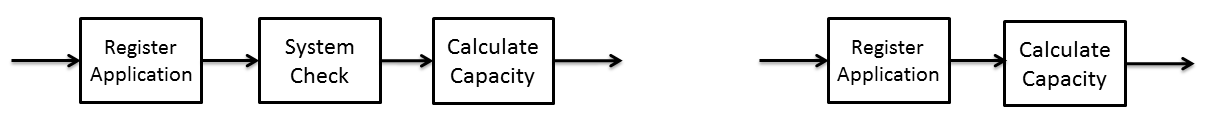
\includegraphics[width=\textwidth]{3_background/mismatch-patterns-skipped-activity}
      \caption{Example of Skipped Activity Pattern}
      \label{fig:skipped-activity}
      \end{figure}
  \item[Refined Activity] An activity exists in one process but, as an equivalent, a collection of activities are existing in the other process to achieve the same task. An illustration is provided in Figure~\ref{fig:refined-activity}. 
      \begin{figure}
      \centering
      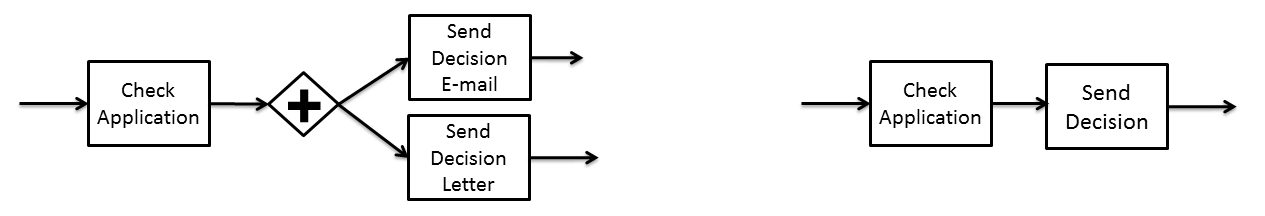
\includegraphics[width=\textwidth]{3_background/mismatch-patterns-refined-activity}
      \caption{Example of Refined Activity Pattern}
      \label{fig:refined-activity}
      \end{figure}
\end{description}
 
Control flow mismatch patterns are based on using different control-flow relations and dependencies for the same activities in different processes. Within the scope of this study, the following related control flow mismatch patterns are defined in study \cite{dijkman2007mismatch}:
\begin{description}
  \item[Activities at Different Moments in Processes] Set of activities are undertaken with different orders in different processes as shown in Figure~\ref{fig:different-moments}. 
      \begin{figure}
      \centering
      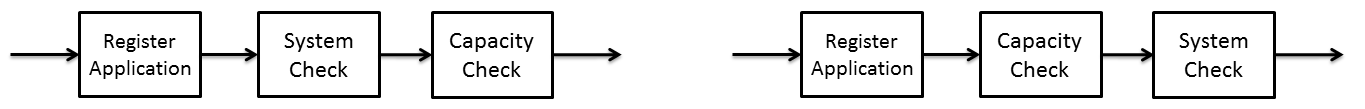
\includegraphics[width=\textwidth]{3_background/mismatch-patterns-different-moments}
      \caption{Example of Activities at Different Moments in Process Pattern}
      \label{fig:different-moments}
      \end{figure}
  \item[Different Conditions for Occurrence] Set of dependencies are same for two processes; however, occurrence condition is different. An example is provided in Figure~\ref{fig:different-conditions}.
      \begin{figure}
      \centering
      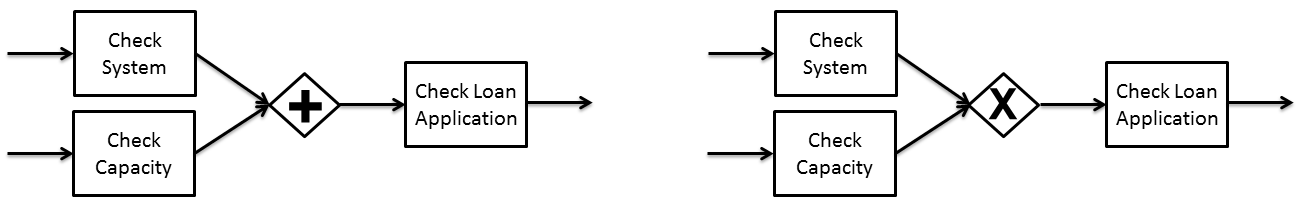
\includegraphics[width=\textwidth]{3_background/mismatch-patterns-different-conditions}
      \caption{Example of Different Conditions for Occurrence Pattern}
      \label{fig:different-conditions}
      \end{figure}
  \item[Different Dependencies] Dependency set of activities differ in different organizations. An example of this pattern is shown in Figure~\ref{fig:different-dependency}.
      \begin{figure}
      \centering
      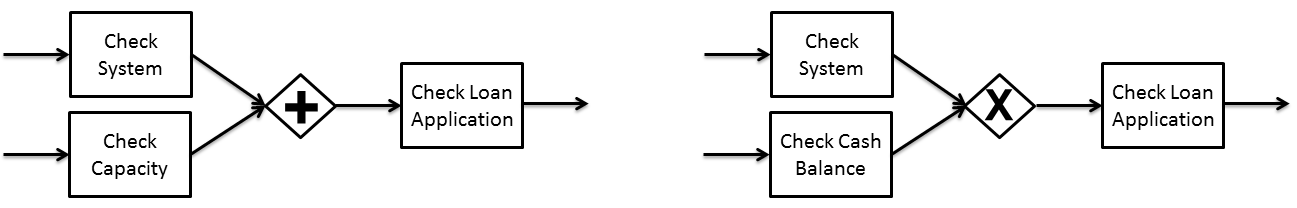
\includegraphics[width=\textwidth]{3_background/mismatch-patterns-different-dependency}
      \caption{Example of Different Dependencies Pattern}
      \label{fig:different-dependency}
      \end{figure}
  \item[Additional Dependencies] This pattern is a special case of different dependencies where one set of activities includes the other and results with additional dependencies as illustrated in Figure~\ref{fig:additional-dependency}.
      \begin{figure}
      \centering
      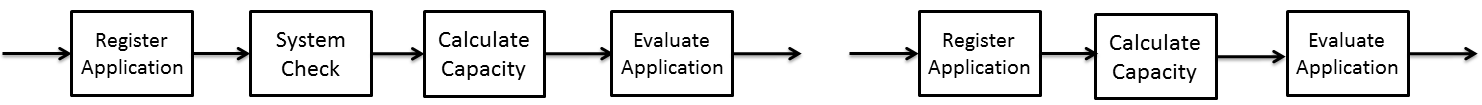
\includegraphics[width=\textwidth]{3_background/mismatch-patterns-additional-dependency}
      \caption{Example of Additional Dependencies Pattern}
      \label{fig:additional-dependency}
      \end{figure}
\end{description}

As mentioned in the study \cite{dijkman2007mismatch}, their approach does not create a comprehensive list to resolve all mismatches but the most common ones spotted during case studies. In addition, from their definitions and examples it can be easily seen that these patterns are not orthogonal. Moreover, there are no algorithms provided to spot these mismatches in \cite{dijkman2007mismatch} or consequent studies, and thus implementation of spotting mismatch patterns are kept within the scope of this thesis study.